%----------
%   WARNING
%----------

% This Guide contains Library recommendations based mainly on APA and IEEE styles, but you must always follow the guidelines of your TFG Tutor and the TFG regulations for your degree.

% THIS TEMPLATE IS BASED ON THE APA STYLE 


%----------
% DOCUMENT SETTINGS
%----------

\documentclass[12pt]{report} % font: 12pt

% margins: 2.5 cm top and bottom; 3 cm left and right
\usepackage[
a4paper,
vmargin=2.5cm,
hmargin=3cm
]{geometry}

% Paragraph Spacing and Line Spacing: Narrow (6 pt / 1.15 spacing) or Moderate (6 pt / 1.5 spacing)
\renewcommand{\baselinestretch}{1.15}
\parskip=6pt

% Color settings for cover and code listings 
\usepackage[table]{xcolor}
\definecolor{azulUC3M}{RGB}{0,0,102}
\definecolor{gray97}{gray}{.97}
\definecolor{gray75}{gray}{.75}
\definecolor{gray45}{gray}{.45}

% In the template we include the file OUTPUT.XMPDATA. You can download that file and include the metadata that will be incorporated into the PDF file when you compile the memoria.tex file. Then upload it back to your project. 
% Commented out due to upstream error
% \use package[a-1b]{pdf}

% LINKS
\usepackage{hyperref}
\hypersetup{colorlinks=true,
	linkcolor=black, % links to parts of the document (e.g. index) in black
	urlcolor=blue} % links to resources outside the document in blue

% MATH EXPRESSIONS
\usepackage{amsmath,amssymb,amsfonts,amsthm}

% Character encoding
\usepackage{txfonts} 
\usepackage[T1]{fontenc}
\usepackage[utf8]{inputenc}

% English settings
\usepackage[spanish]{babel} 
\usepackage[babel, spanish=spanish]{csquotes}
\AtBeginEnvironment{quote}{\small}

% Footer settings
\usepackage{fancyhdr}
\pagestyle{fancy}
\fancyhf{}
\renewcommand{\headrulewidth}{0pt}
\rfoot{\thepage}
\fancypagestyle{plain}{\pagestyle{fancy}}

% DESIGN OF THE TITLES of the parts of the work (chapters and epigraphs or sub-chapters)
\usepackage{titlesec}
\usepackage{titletoc}
\titleformat{\chapter}[block]
{\large\bfseries\filcenter}
{\thechapter.}
{5pt}
{\MakeUppercase}
{}
\titlespacing{\chapter}{0pt}{0pt}{*3}
\titlecontents{chapter}
[0pt]                                               
{}
{\contentsmargin{0pt}\thecontentslabel.\enspace\uppercase}
{\contentsmargin{0pt}\uppercase}                        
{\titlerule*[.7pc]{.}\contentspage}                 

\titleformat{\section}
{\bfseries}
{\thesection.}
{5pt}
{}
\titlecontents{section}
[5pt]                                               
{}
{\contentsmargin{0pt}\thecontentslabel.\enspace}
{\contentsmargin{0pt}}
{\titlerule*[.7pc]{.}\contentspage}

\titleformat{\subsection}
{\normalsize\bfseries}
{\thesubsection.}
{5pt}
{}
\titlecontents{subsection}
[10pt]                                               
{}
{\contentsmargin{0pt}                          
	\thecontentslabel.\enspace}
{\contentsmargin{0pt}}                        
{\titlerule*[.7pc]{.}\contentspage}  


% Tables and figures settings
\usepackage{multirow} % combine cells 
\usepackage{caption} % customize the title of tables and figures
\usepackage{floatrow} % we use this package and its \ ttabbox and \ ffigbox macros to align the table and figure names according to the defined style.
\usepackage{array} % with this package we can define in the following line a new type of column for tables: custom width and centered content
\newcolumntype{P}[1]{>{\centering\arraybackslash}p{#1}}
\DeclareCaptionFormat{upper}{#1#2\uppercase{#3}\par}
\usepackage{graphicx}
\graphicspath{{../imagenes/}} % images folder

% Table layout for social sciences and humanities
\captionsetup*[table]{
	justification=raggedright,
	labelsep=newline,
	labelfont=small,
	singlelinecheck=false,
	labelfont=bf,
	font=small,
	textfont=it
}

% Figure layout for social sciences and humanities
\captionsetup[figure]{
	%name=Figura,
	singlelinecheck=off,
	labelsep=newline,
	font=small,
	labelfont=bf,
	textfont=it
}
\floatsetup[figure]{
    style=plaintop,
    heightadjust=caption,
    footposition=bottom,
    font=small
}

% Figures and tables footnote layout 
\captionsetup*[floatfoot]{
    footfont={small, up}
}

% FOOTNOTES
\usepackage{chngcntr} % continuous numbering of footnotes
\counterwithout{footnote}{chapter}

% CODE LISTINGS 
% support and styling for listings. More information in  https://es.wikibooks.org/wiki/Manual_de_LaTeX/Listados_de_código/Listados_con_listings
\usepackage{listings}

% Custom listing
\lstdefinestyle{estilo}{ frame=Ltb,
	framerule=0pt,
	aboveskip=0.5cm,
	framextopmargin=3pt,
	framexbottommargin=3pt,
	framexleftmargin=0.4cm,
	framesep=0pt,
	rulesep=.4pt,
	backgroundcolor=\color{gray97},
	rulesepcolor=\color{black},
	%
	basicstyle=\ttfamily\footnotesize,
	keywordstyle=\bfseries,
	stringstyle=\ttfamily,
	showstringspaces = false,
	commentstyle=\color{gray45},     
	%
	numbers=left,
	numbersep=15pt,
	numberstyle=\tiny,
	numberfirstline = false,
	breaklines=true,
	xleftmargin=\parindent
}

\captionsetup*[lstlisting]{font=small, labelsep=period}
 
\lstset{style=estilo}
\renewcommand{\lstlistingname}{\uppercase{Código}}


% REFERENCES 

\usepackage{color}

% used for cite command, and changing the color the URL and dates are.
\usepackage{hyperref} 
\hypersetup{
    colorlinks=true,
    linkcolor=blue,
    urlcolor=blue,
    linktoc=all,
    citecolor=black
           }

% APA bibliography setup
\usepackage[style=apa, backend=biber, natbib=true, hyperref=true, uniquelist=false, sortcites]{biblatex}

\addbibresource{referencias.bib} % The references.bib file in which the bibliography used should be

% Caption package, for use of subfigures.
\usepackage{subfig}

% Create a list of glossaries and acronyms
\usepackage[acronym]{glossaries}
\makeglossaries

%-------------
%	DOCUMENT
%-------------

\begin{document}

\pagenumbering{roman} % Roman numerals are used in the numbering of the pages preceding the body of the work.
	
%----------
%	COVER
%----------	
\begin{titlepage}
	\begin{sffamily}
  \begin{figure}%
    \raggedleft
    \subfloat{{
\includegraphics[width=3cm]{UNED.jpg} }}%
    \hspace*{\fill}
    \subfloat{{
\includegraphics[width=5cm]{Scalefast.jpg} }}%
\end{figure}
	\begin{center}
		\vspace{2.5cm}
		\begin{Large}
			Master en Ciberseguridad\\			
			 2020-2021\\
			\vspace{2cm}		
			\textsl{Trabajo de final de Master}
			\bigskip
			
		\end{Large}
		 	{\Huge ``Definicion, creacion e implementaicon del SecDevOps''}\\
		 	\vspace*{0.5cm}
	 		\rule{10.5cm}{0.1mm}\\
			\vspace*{0.9cm}
			{\LARGE Sergio Rosello Morell}\\ 
			\vspace*{1cm}
		\begin{Large}
			David Aracil Cofrade\\
			Rafael Pastor Vargas\\
			Madrid, a \today \\
		\end{Large}
	\end{center}
	\vfill
	\color{black}
	\fbox{
	\begin{minipage}{\linewidth}
    	\textbf{AVOID PLAGIARISM}\\
    	\footnotesize{The University uses the \textbf{Turnitin Feedback Studio} for the delivery of student work. This program compares the originality of the work delivered by each student with millions of electronic resources and detects those parts of the text that are copied and pasted. Plagiarizing in a TFM is considered a  \textbf{\underline{Serious Misconduct}}, and may result in permanent expulsion from the University.}\end{minipage}}

	% IF OUR WORK IS TO BE PUBLISHED UNDER A CREATIVE COMMONS LICENSE, INCLUDE THESE LINES. IS THE RECOMMENDED OPTION.
	\noindent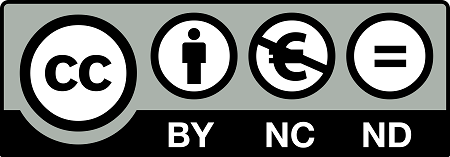
\includegraphics[width=4.2cm]{creativecommons.png}\\ % Creative Commons Logo
    \footnotesize{This work is licensed under Creative Commons \textbf{Attribution – Non Commercial – Non Derivatives}}
	
	\end{sffamily}
\end{titlepage}

\newpage % blank page
\thispagestyle{empty}
\mbox{}




%----------
%	ABSTRACT AND KEYWORDS 
%----------	
\renewcommand\abstractname{\large\bfseries\filcenter\uppercase{Sumario}}
\begin{abstract}
\thispagestyle{plain}
\setcounter{page}{3}
	
Inicio del movimiento DevOps, el 2010, con el desarrollo agil\\
Adopcion de la cultura agil por silicon valley y resto de munto\\
Implementacion de seguridad dentro del desarrollo agil\\
Uso de Pipelines, para desarrollar SW con la seguridad en mente\\
Caso especifico de la implementacion en Scalefast\\
\vfill
\end{abstract}
	
\newpage % Blank page
\renewcommand\abstractname{\large\bfseries\filcenter\uppercase{Abstract}}
\begin{abstract}
\thispagestyle{plain}
\setcounter{page}{5}

Start of Agile SW development, and DevOps culture\\
Adoption of culture by Silicon Valley and subsequent popularization\\
Security inside agile development?\\
Use of Pipelines in security-focused Agile development\\
Specific case with Scalefast\\

\textbf{Palabras clave:} % add the keywords
	
\vfill
\end{abstract}
\newpage % Blank page
\thispagestyle{empty}
\mbox{}


%----------
%	Dedication
%----------	
\chapter*{Agradecimientos}

\setcounter{page}{7}
	
Agradecer principalmente este trabajo a:

\begin{itemize}
  \item{Familia}
  \item{Tutores}
  \item{UNED}
  \item{Scalefast}
\end{itemize}

		
	\vfill
	
	\newpage % blank page
	\thispagestyle{empty}
	\mbox{}
	




%----------
%	TOC
%----------	

%--
% TOC
%-
\tableofcontents
\thispagestyle{fancy}

\newpage % blank page
\thispagestyle{empty}
\mbox{}




%--
% List of figures. If they are not included, comment the following lines
%-
\listoffigures
\thispagestyle{fancy}

\newpage % blank page
\thispagestyle{empty}
\mbox{}




%--
% List of tables. If they are not included, comment the following lines
%-
\listoftables
\thispagestyle{fancy}

\newpage % blankpage
\thispagestyle{empty}
\mbox{}





\newglossaryentry{job}
{
        name=job,
        description={Proceso ejecutado automáticamente, a partir de un evento externo, varios jobs ordenados de forma lógica forman un pipeline}
}
\newglossaryentry{API}
{
        name=Application Programming Interface, description={Permite que un
        servicio y un producto se comuniquen, permitiendo al producto crear una
        funcionalidad usando la información que proporciona el servicio a través
        de una interfaz estipulada.  Los desarrolladores no necesitan saber como
        se ha implementado el servicio, solamente, como se usa, para obtener la
        información requerida.}
}
\newglossaryentry{staging}
{
        name=staging,
        description={Un entorno que reproduce exactamente el entorno de producción cuya finalidad es asegurar que el código que se va a desplegar en producción funcione correctamente}
}
\newglossaryentry{App-Sec}
{
        name=Application Security,
        description={El dominio de la seguridad de la aplicación dentro del 
        sector de la seguridad.}
}
\newglossaryentry{DevOps}
{
        name=DevOps,
        description={Un nivel de abstracción superior al desarrollo ágil cuya
        finalidad es conseguir una sinergia entre personas, procesos y
        herramientas}
}
\newglossaryentry{STRIDE}
{
        name=STRIDE,
        description={Un acrónimo en lengua inglesa para las siguientes palabras:
        Spoofing, Tampering, Repudiation, Information Disclosure, Denial of
        service y Elevation of privilege}
}
\newglossaryentry{DevSecOps}
{
        name=DevSecOps,
        description={Una inclusion de las herramientas de seguridad en la
        filosofía DevOps}
}
\newglossaryentry{PenTest}
{
        name=PenTest,
        description={Una serie de revisiones manuales o automáticas que se
        realizan contra una pagina web o servicio expuesto públicamente en
        Internet cuya
        finalidad es vulnerar dicha pagina o servicio}
}
\newglossaryentry{pipeline}
{
        name=pipeline,
        description={Serie de procesos automatizados que realizan comprobaciones automatizadas sobre el programa que se pretende desplegar en el entorno de producción}
}

\newacronym{SDLC}{SDLC}{Software Development Life Cycle}
\newacronym{mr}{MR}{Merge Request}


%----------
%	THESIS
%----------	
\clearpage
\pagenumbering{arabic} % numbering with Arabic numerals for the rest of the document.	

\chapter{Estado del arte}

\section{Evolución del desarrollo de software, desde su concepción hasta la actualidad}

Hablar del desarrollo del software desde su concepción hasta su actualidad require especial atención ya que el software solo es posible gracias al hardware sobre el que se ejecuta.
Naturalmente, este campo ha adoptado las costumbres y características del mundo del Hardware.

Para entender la evolución del software, nos tenemos que remontar a los años cincuenta de la década pasada, en la que mantener un ordenador suponía un gasto enorme debido a que el software que corría en el ordenador estaba tan acoplado al hardware sobre el que corría, que cada ordenador tenia su propio lenguaje de programación. 
No fue hasta 1957 que se desarrollo FORTRAN, el primer lenguaje de programación, creando así el primer estándar de lenguaje de programación. FORTRAN 66 \cite{FORTRAN1966}.
Al no disponer de una conexión a Internet y requerir la presencia de ingenieros enviados por parte de la compañía que fabrica el propio ordenador, las empresas que poseían un ordenador, no esperaban tener que actualizar su software regularmente.
A medida que se avanzaba en la fabricación de ordenadores personales y se estandarizaba Internet, los requisitos para poder actualizar el software del ordenador empezaban a ofrecer menos resistencia.

Pasamos del inicio de los lenguajes de programación al inicio de los comercios en Internet.
A medida que evoluciona Internet, también lo hacen las aplicaciones que se alojan en el, pasamos de Internet 1.0, a  Internet 2.0, en el que las paginas web dejan de ser portales de visita, como revistas, y se empieza a poder diferenciar clientes, y adaptar el funcionamiento de la pagina al cliente especifico.
Estos nuevos requisitos, incorporan nueva complejidad a la ya creciente complejidad del software, como por ejemplo, cualquier pagina que tenga que poder diferenciar a sus clientes, por lógica de negocio, debe añadir a su pila de componentes, una base de datos.

Debido a esta creciente complejidad, las empresas cuyo modelo de negocio estaba basado en el software, ofrecían actualizaciones muy poco regularmente ya que a mayor complejidad de aplicación, mayor era el tiempo que se tenia que designar a la compilación de las distintas piezas que componían el software. (Base de datos, Portal frontal, Sistema de lógica interna, entre otras.)
Es por esto que el proceso de Despliegue ha sido y sigue siendo uno de los puntos de estrés de muchas empresas.

La realidad, es que desde 1957, en el que se pretendía desarrollar iterativamente e incrementalmente \cite{IID}, se ha estado pensando colectivamente en como mejorar el desarrollo de software, desde su fase de concepción, a su fase de despliegue.
No obstante, no es hasta 2001 cuando se escribió el manifesto del desarrollo ágil \cite{agile}, en el que se destacan los pilares fundamentales sobre los que se ha construido la filosofía DevOps \cite{CD-TF}, posteriormente extendida a la filosofía DevSecOps.

En conclusion, saber a cerca de la evolución del software facilita también la comprensión de los objetivos de este trabajo que se resumen en: <++> %TODO: List TFG objectives.


\subsection{Historia de los despliegues}

En esta sección analizaremos las distintas formas en las que se ha desarrollado software comúnmente, hasta hoy en día, haciendo énfasis en el desarrollo ágil, y el uso de \Gls{pipeline}s para garantizar cierta calidad del software antes de desplegar.

Así pues, en la década de 1950, se empieza a pensar y desarrollar una mejor forma de construir software.
El proyecto más memorable en el que se hace uso de técnicas modernas de desarrollo de software es "Project Mercury".
Este proyecto, centrado en poner al hombre a la luna, requería de una capacidad de construcción de software ejemplar.
Gerald M. Weinberg fue el arquitecto del proyecto.
Decidieron que ``el desarrollo en cascada aplicado a un proyecto grande era bastante estúpido, o al menos, ignorante a la realidad'' \cite{GW-PM} y desarrollaron software con una metodología similar a la estipulada por XP. \cite{XP}

No es sin embargo hasta 1968 cuando encontramos la primera aparición formal de desarrollo iterativo, que aparece en un documento interno de IBM en el que se describe que primero se define formalmente la funcionalidad, posteriormente se establecen unos tests, y se empieza a desarrollar, a medida que avanza el proceso, se crean nuevos tests, mas específicos, al final, el sistema, se convierte en la aplicación. \cite{ID-FB}

En los años setenta, se documenta por primera vez el desarrollo en cascada en el articulo que escribe el Dr. Winston W. Royce.
Como curiosidad, Royce aconseja realizar el proceso de desarrollo compuesto por las fases de análisis de requisitos, construcción del software, testeo y despliegue dos veces, pero a medida que se ha extendido esta metodología, se ha popularizado siguiendo únicamente una de estas iteraciones, quedando en el desarrollo en cascada que se conoce hoy en día. \cite{royce1970}
Esta metodología adaptada, heredada del articulo del Dr. Winston W. Royce sobre como desarrollar software, se popularizo enormemente, a pesar de sus desventajas en cuanto a flexibilidad, adaptabilidad y estimación de tiempos.

Otro notable proyecto que describe la forma en la que se han llevado a cabo sus fases de desarrollo de software, es el desarrollo de una familia de compiladores extendidos para una familia de lenguajes de programación específicos a dominio.
En este articulo, se describe claramente el desarrollo iterativo incremental (IID). \cite{6312870}

Durante los años 70, el desarrollo en cascada cobra una popularidad abismal, tanta, que los lideres de equipo encargados de proyectos tan importantes como la creación del software de la lanzadera espacial de la NASA, sentían la obligación de justificar por que no habían usado el método de de desarrollo en cascada.
La justificación mas común para no usar el desarrollo en cascada, era que los requisitos del proyecto cambiaban continuamente, y no podían ajustar el desarrollo en cascada a estos cambios.

En los años 80, muchos desarrolladores prominentes publican artículos sobre como el desarrollo en cascada no es una buena forma de construir un proyecto medianamente grande de software.
Parafraseando el articulo titulado ``Un proceso de diseño racional: Como y por que falsearlo'' \cite{Parnas1986}
\begin{itemize}
  \item{Un usuario raramente sabe exactamente todo lo que quiere y no puede expresar todo lo que sabe}
  \item{Existen muchos detalles de implementación que no se pueden anticipar, aunque tengamos todos los requisitos claros}
  \item{Aunque sepamos todos los detalles, como humanos, no podemos procesar tanta complejidad}
  \item{Aunque pudiésemos procesar toda esta complejidad, existen fuerzas exteriores, que hacen que cambien los requisitos o invaliden decisiones previas}
\end{itemize}
Estas razones encabezan la lista de motivos por los que la tendencia a la hora de desarrollar software debía de virar hacia el desarrollo incremental e iterativo.

Desde los años 90 hasta la actualidad, a medida que el desarrollo en cascada demostraba que no era lo suficientemente flexible para llevar a cabo proyectos medianamente grandes, cantidad de nuevos artículos aparecían con nuevas y mejoradas técnicas de desarrollo iterativo e incremental.
Muchas de estas siguen aplicándose hoy en día, como XP (Extreme Programming), Dynamic Systems Development Method (DSDM), Scrum y FDD (Feature Driven Development), entre otras.
El 1 de febrero de 2001, se celebra una reunion entre varios expertos en procesos, entre ellos, los promotores de XP, Scrum, FDD. 
En ese momento se forma la alianza ágil (agile alliance), cuya función es promover métodos de desarrollo de software iterativo e incremental. 

\section{Desarrollo ágil}

Como se ha reverenciado anteriormente, el desarrollo ágil forma parte del ADAN del desarrollo de software.
Muchos de los proyectos mas complejos se han construido usando técnicas que recuerdan mucho a la metodología ágil. \cite{GW-PM}
Afortunadamente, a medida que nos adentramos en la actualidad, podemos observar como el uso de la metodología ágil aumenta en popularidad \cite{Hoyada}.
A día de hoy, el 95\% de las empresas dicen desarrollar software siguiendo la metodología ágil. \cite{stateofagile}

\subsection{Que es el desarrollo ágil}

El termino ``Desarrollo Ágil'' se acuñó en 2001, en una reunion que celebraron distintos representares de alternativas al popular desarrollo en cascada.
En esta reunion, asistieron representares de técnicas de desarrollo como Extreme Programming, SCRUM, DSDM, Adaptive Software Development, Crystal, Feature-Driven Development, Pragmatic Programming y otros simpatizantes.
La finalidad era asentar unas bases sobre las que todos estuviesen de acuerdo.

Al terminar, se acuñó el término desarrollo ágil.

Los principales valores del desarrollo ágil son los siguientes: \cite{agilePrinciples}

\begin{itemize}
  \item{Nuestra mayor prioridad es satisfacer al cliente mediante la entrega temprana y continua de software con valor.}
  \item{Aceptamos que los requisitos cambien, incluso en etapas tardías del desarrollo. Los procesos Ágiles aprovechan el cambio para proporcionar ventaja competitiva al cliente.}
  \item{Entregamos software funcional frecuentemente, entre dos semanas y dos meses, con preferencia al periodo de tiempo más corto posible.}
  \item{Los responsables de negocio y los desarrolladores trabajamos juntos de forma cotidiana durante todo el proyecto.}
  \item{Los proyectos se desarrollan en torno a individuos motivados. Hay que darles el entorno y el apoyo que necesitan, y confiarles la ejecución del trabajo.}
  \item{El método más eficiente y efectivo de comunicar información al equipo de desarrollo y entre sus miembros es la conversación cara a cara.}
  \item{El software funcionando es la medida principal de progreso.}
  \item{Los procesos Ágiles promueven el desarrollo sostenible. Los promotores, desarrolladores y usuarios debemos ser capaces de mantener un ritmo constante de forma indefinida.}
  \item{La atención continua a la excelencia técnica y al buen diseño mejora la Agilidad.}
  \item{La simplicidad, o el arte de maximizar la cantidad de trabajo no realizado, es esencial.}
  \item{Las mejores arquitecturas, requisitos y diseños emergen de equipos auto-organizados.}
  \item{A intervalos regulares el equipo reflexiona sobre cómo ser más efectivo para a continuación ajustar y perfeccionar su comportamiento en consecuencia.}
\end{itemize}

\subsection{Como llevar a cabo el desarrollo ágil}

Una vez repasados los valores del desarrollo ágil, debemos ahondar más en como repercuten estos en el día a día de un proyecto de software que usa la metodología ágil.

Cada uno de los pasos descritos a continuación forma parte de una iteración dentro del proceso de desarrollo de software.
Estas fases, van construyendo sobre las previas, hasta que se completa la aplicación.

\subsubsection{Firma del contrato}

Al inicio de la colaboración, se tiene una reunion, en la que el cliente y la empresa trabajan conjuntamente para asentar las bases sobre las que se construirá el proyecto.
Este tipo de enfoque se llama ``top-down approach'' %TODO: Cite needed

\subsubsection{tests de aceptación}

Una vez establecidas ciertas bases, se empiezan a definir funcionalidades, casos de uso.
Aquí es donde entran en juego técnicas de verificación de los casos de uso.
Se generan documentos ejecutables que consisten en asentar los requisitos básicos para que un usuario realize una acción y llegue a un resultado final esperado, dadas unas pre condiciones.
Estos tests, se llaman comúnmente tests de aceptación, y se encargan de verificar que el software realizado por la empresa cumple con los requisitos impuestos por el cliente.

El desarrollador puede saber cuando ha acabado de implementar el ``happy path'' de su parte del código cuando su trabajo pasa todos los tests de aceptación que se han definido con anterioridad.
La ventaja que tienen estos tests frente al resto de tests que se usan de desarrollo ágil, es que estos tests están diseñados para que cualquier persona, sea desarrollador, o no, los pueda definir, crear, y editar.
De esta forma, el desarrollo se mantiene ágil iteración tras iteración, ya que en caso de haber un cambio entre iteraciones, únicamente se tienen que ejecutar los tests de aceptación para saber si la version actual del software cumple con los nuevos requisitos.

La sintaxis estándar de los tests de aceptación es la siguiente:

\begin{lstlisting}
Feature: Registro de usuario

  Background:
    Given la base de datos esta actualizada

  Scenario: Usuario existente inicia sesion
    Given ya tengo cuenta en la aplicacion
    When introduzco mis credenciales correctamente
    Then inicio sesion en la aplicacion
\end{lstlisting}

De esta forma, se definen las características (``Features'') del producto a construir.
Cada característica engloba una serie de ``caminos felices'' que puede seguir el usuario.
La concatenación de acciones que sigue el usuario para llegar a un estado final se llama ``camino feliz'' (``Scenario'').
Dentro de cada camino feliz, existen una serie de acciones, representadas por ``Given, When y Then''.

\begin{itemize}
  \item{``Given'' representa el estado inicial en el que debe estar la aplicación}
  \item{``When'' representa la acción a ejecutar}
  \item{``Then'' representa el estado final en el que debe quedar la aplicación.}
\end{itemize}

Este estilo, o formato de escritura se denomina ``Gherkin'' y es fundamental en la vertiente BDD de desarrollo ágil.

\subsubsection{Desarrollo y testeo del código}

Una vez se ha definido la especificación, los programadores, pueden empezar con el desarrollo.
Esto asegura que todo el mundo trabaja en sincronía, desde los clientes, al analista, al jefe de proyecto, al desarrollador.
La existencia de estos tests hace que cualquier persona involucrada en el proyecto que quiera revisar la documentación se dirija al mismo sitio.
Esto obliga a que esta documentación viviente, se mantenga actualizada y al día, entre iteraciones.

A medida que los programadores ahondan en complejidad de desarrollo, se encuentran con una complejidad cada vez mayor.
Siguiendo con el ejemplo anterior, del inicio de sesion, se tienen que definir casos mas específicos, como la forma en la que se conecta la plataforma a la base de datos, el mensaje de error que aparece cuando el nombre de usuario es incorrecto, y cuando la contraseña es incorrecta, entre muchos otros.
Para asegurar el correcto funcionamiento de su código, los desarrolladores deben crear tests para cubrir cualquier cauce que pueda tomar su código.
De esta forma, pueden delegar la comprobación de su código a los tests, que van a verificar que la lógica que están programando es la adecuada, definida previamente.
Una vez se hayan ejecutado los tests, el programador puede estar seguro de que ha implementado correctamente el código que se le ha solicitado crear.

Existe un nivel mas detallado de tests.
Estos se llaman tests unitarios.
Su función es validar el correcto funcionamiento de los componentes específicos (Funciones, clases, datos) y la forma  que tienen de alterar o crear los datos necesarios, que, en combinación unos con otros, habilitan la creación de la lógica de la aplicación.

\subsubsection{Despliegue del código}

Una vez los desarrolladores han terminado la tarea, y el proyecto cumple con las especificaciones descritas por el cliente, es hora de desplegar el código a producción.

Al centrarse principalmente en la fase de desarrollo de software, los equipos que siguen las recomendaciones estipuladas por la metodología ágil, frecuentemente olvidan la importancia del despliegue en el flujo de desarrollo del software y el despliegue, deja de ser parte del proceso iterativo, sino que, al terminar el desarrollo, se despliega el código a producción.

Esta ha sido el modus operandi de la mayoría de equipos que han seguido el desarrollo ágil.

Esto desemboca en tremendos dolores de cabeza que pueden llegar a prolongarse durante horas para pasar el código desarrollado en los equipos internos de la empresa a los equipos destinados para alojar el código en producción o que directamente pueden llevar a una empresa a la bancarrota en cuestión de minutos. \cite{seven2014}

\section{De desarrollo ágil, a DevOps}

Llegados a este punto, hay que tener en cuenta que para llevar a cabo cualquier tipo de proyecto, deben haber como mínimo dos partes implicadas.
El cliente y la empresa que va a llevar a cabo la vision del cliente.
Estas dos partes pueden ser tan complejas o simples como se quiera, pero deben existir.
Desde un proyecto llevado a cabo únicamente por una persona a un proyecto distribuido separado entre distintas zonas horarias.

La mayor de las responsabilidades del \textbf{cliente} es especificar claramente los requisitos del producto o idea que tiene en mente.
La responsabilidad de \textbf{la empresa} es de desarrollar el producto que tiene el ciente en mente lo mas fielmente posible.
La clave del éxito del desarrollo ágil, basado en iteraciones incrementales, es que establece canales de comunicación directos, estrechos e iterativos entre el cliente y la empresa.
(Existen modelos de desarrollo ágil, en el que se recomienda que el cliente comparta habitación con la empresa que esta desarrollando su producto)

Aunque, como ya se ha demostrado en empresas no directamente relacionadas con el mundo del Software como Canon, Honda, o NEC, entre otras, se puede aplicar el desarrollo ágil a cualquier sector \cite{Hirotaka1986}.
En el mundo del software, podemos hacer uso de herramientas automatizadas y frameworks para satisfacer los principales valores del desarrollo ágil.
De esta forma, se logra crear un proyecto que se mantiene actualizado entre las especificaciones y el desarrollo.

En 2006, se escribe públicamente por primera vez sobre este proceso, en el articulo llamado ``The Deployment Production Line'' en el que se describe como construir una cadena de montaje, en la que el código puede ser desplegado a producción sencillamente presionando un botón, y revertido, en caso de que algo fuera mal de igual manera. \cite{10.1109/AGILE.2006.53}

\subsection{Que es DevOps}


La filosofía DevOps nace como respuesta a una falta de comunicación, y creciente frustración entre equipos dentro de un mismo desarrollo.

Su finalidad es establecer una comunicación constante entre las distintas fases y equipos de desarrollo, mayoritariamente entre los desarrolladores y los equipos de operaciones, que se encargan de poner el código que genera el equipo de desarrolladores a un entorno de producción. Esto no quiere decir que se excluyan a cualquier otro equipo involucrado en el desarrollo del software, como el de QA.

El fenómeno DevOps se puede considerar una extension del desarrollo ágil, debido a que, en su forma mas reducida, acorta las iteraciones del desarrollo de una fecha especifica, a un commit especifico. \cite{dobra2018}
Cada commit pasa por una serie de comprobaciones o ``jobs'' dentro de un ``pipeline'' para verificar que efectivamente el código que se quiere añadir a producción es adecuado para ser desplegado.

Otras de las prioridades de la cultura DevOps es Habilitar la automatización sobre la documentación, presentar al desarrollador posibilidades (API de testeo de código), en vez de impedimentos (procesos)

Como consecuencia, se crea un flujo automatizado de Integración Continua y Despliegue Continuo del código generado iterativamente a lo largo de todo el proyecto. Este flujo se llama ``Pipeline''.

La filosofía DevOps en la construcción y despliegue de software, por tanto gira en torno a establecer una serie de procesos y comprobaciones por los que tiene que pasar cada desarrollo candidato a se desplegado a producción. 

Desde la concepción del proyecto, antes de desarrollar el código, se establecen los pasos mínimos por los que tiene que pasar cada candidato a producción (commit) creando así un ``Pipeline'', que es la union de esos pasos automatizados, de forma que, para que el candidato a producción llegue a producción, siempre tenga que pasar por estos mismos pasos y comprobaciones.
Ya sea un apaño en producción, como un desarrollo nuevo.

En la metodología ágil, el desarrollo de una nueva funcionalidad se hace de forma iterativa e incremental, empezando primero por los tests.
En el enfoque de la filosofía DevOps, la creación del Pipeline se añade anteriormente a los tests, para que, una vez se este desarrollando, se puedan revisar los desarrollos directamente con los tests, de forma automática en el Pipeline una vez se cumplen una serie de acciones, normalmente, un commit.

Al igual que en el desarrollo ágil, el desarrollo del Pipeline es siempre constante, este también va creciendo de forma iterativa e incremental, añadiendo más tests, más pasos, y por tanto revisando y asegurando mayor confianza en el commit que pasa todo el pipeline.

En esencia, se trata de un desarrollo mas, pero en vez de que su función sea cumplir un requisito del cliente, su función es asegurar la estabilidad y calidad del software entregado al cliente. 

``Cada vez que se añade un cambio al servidor de control de versiones, se espera que pase todos los tests, produzca código funcional y se pueda desplegar a producción.
Esta es la suposición inicial.
La tarea de un sistema de integración continua es la de refutar dicha suposición, demostrando que este candidato a producción no es adecuado para entrar a producción''\cite{Humble2010}

En el libro ``Accelerate'', de Nicole Forsgren, Jez Humble y Gene Kim, los autores comentan que la diferencia entre una gran empresa y una pequeña y mediana empresa, es que las grandes empresas siguen cuatro indicadores de compromiso muy de cerca, y se han bulto expertas en reducir al máximo estos mismos.
Los indicadores de compromiso son: el plazo de entrega, la frecuencia de despliegue, el tiempo medio en restaurar (MTTR) y el porcentaje de cambio vs error.\cite{Forsgren2018}

Una filosofía DevOps es clave para reducir estos indicadores.
Con el uso de ``Pipelines'' y cambiando la cultura de la empresa, facilitando a los desarrolladores herramientas y creando flujos y políticas para que estos indicadores vayan reduciendo el tiempo medio, implica que la empresa el question tiene un potencial enorme y, por consiguiente una ventaja competitiva sobre sus competidores.

\section{De DevOps a DevSecOps}

La seguridad en la metodología ágil no ha sido especialmente contemplada durante la popularización de este tipo de desarrollo, sin embargo, la metodología ágil destaca por su modularidad, y capacidad de reacción frente a cambios de requisitos, o nuevas prioridades en el proyecto.
Al poder adaptarse a nuevas vertientes y filosofías, como la de DevOps, se forman distintas expresiones de desarrollo ágil, cada una enfatiza en su propia metodología, pero todas parten de ma misma base. \cite{agilePrinciples}.

\subsection{La seguridad desde un punto de vista clásico}
 
La seguridad en el mundo del software ha estado relegada a un plano inferior debido a que normalmente no ha sido necesaria para el desarrollo del producto agenciado.
Al mismo tiempo, durante los años 90 cuando el contenido que alojaban las paginas web en Internet era mayoritariamente estático, y no estaba disponible a muchos usuarios, la seguridad era una pieza del puzzle que no estaba contemplada, ya que los usuarios no tenían forma de interactuar con la web.
Se parecía, por tanto, a un libro, cuyo contenido esta disponible al lector una vez ha sido impreso.
La primera vez que se hace referencia a la nueva web 2.0 es en el articulo titulado ``Fragmented Future'', en el que se describe el cambio de paradigma que surgirá en la web, a partir de 1999 y se pasa de tener paginas web estáticas a aplicaciones web, en las que los usuarios van a interactuar con el contenido. \cite{DiNucci1999}
En el desarrollo de estas aplicaciones web, los desarrolladores implementaban las funcionalidades sin pensar en como otra gente pudiese romper la aplicacion para sacar provecho del sistema en el que corre, independientemente de la naturaleza y sector de la aplicacion.

No obstante, a medida que la tecnología ha avanzado, ha permitido a las empresas crear modelos de negocio de giraba en torno a Internet.
Un ejemplo bastante conocido puede ser en caso de Amazon.
Estas empresas ofrecen su servicio, su valor a través de una pagina web, y los clientes deben estar identificados para poder obtener los beneficios que ofrecen estas empresas.
Para llevar a cabo el modelo de negocio anterior, dichas empresas deben tener la capacidad de identificar a los clientes, por tanto se deben almacenar datos personales.
Estos datos tienen un gran valor para los hackers, que luego pueden venderlos en el mercado negro.
A medida que Internet se ha extendido, se ha demostrado que hay gente que ha utilizado dicho factor para sacar un beneficio personal.

El sector del software ha intentado mitigar, o prevenir los ataques de ciberseguridad mediante iniciativas como por ejemplo programas de recompensa a la gente que les reporta dichos fallos o vulnerabilidades.
Estos programas se llaman: ``Threat Bounty Programs''
Por lo general, los requisitos de seguridad se mantienen separados de otros requisitos de sistema, por tanto, no se integran en la estrategia general de desarrollo de software. \cite{Flec2003}
Esto quiere decir que los productos que no se han desarrollado con la seguridad en mente, son mas vulnerables a su explotación.
Las desventajas de esta metodología de desarrollo son varias, desde una potencial sanción, si se tratan datos sensibles de usuarios, hasta una explotación de los servicios que ofrece la empresa para beneficio del individuo.
Cabe destacar la ausencia de cualquier aspecto relacionado con la seguridad en el paper que popularizo el desarrollo en cascada. \cite{royce1970}

El sector de la seguridad ha ido creciendo en popularidad desde 1999, en el que se funda el CVE (Common Vulnerabilities and Exposures). 
Entonces, el campo de la ciberseguridad ha sido relegado al mantenimiento de la aplicacion una vez lanzada, pero actualmente la industria ha ido identificando la importancia de la seguridad a nivel de desarrollo y ha ido fomentando esta práctica, con filosofías como la de DevSecOps para convertirse en una parte fundamental del proceso de desarrollo de software ágil de hoy en día.

\subsection{Que es DevSecOps}

Siguiendo la inercia del movimiento DevOps, adoptado al inicio por grandes empresas y seguido de medians y pequeñas empresas, DevSecOps es una extension de la misma filosofía, reconociendo a la seguridad de la aplicacion y del entorno en el que se ejecuta como un factor igual de importante en el ciclo de vida del software.

El propósito de este movimiento es concienciar a los desarrolladores de la importancia del desarrollo seguro de código, principalmente, cambiando la cultura de la empresa, para que los desarrolladores tengan el cuenta la seguridad en el momento en el que desarrollan la aplicacion.

Al igual que en el movimiento DevOps, esto se puede conseguir mediante la incorporación de ``Jobs'' que revisen el estado del código generado durante el desarrollo.
Aun así, la mejor forma de seguir esta filosofía es creando una cultura que la reconozca y respalde, de forma que los desarrolladores no se molestan al ver que el código tiene vulnerabilidades, sino que evolucionen, mediante formaciones o reportes de los fallos de su código, a desarrollar de forma segura.

El ciclo de vida del software, consiste en cinco fases: Planificación, Análisis, Diseño, Implementación y Mantenimiento.

%TODO: Añade gráfico del ciclo de vida del software.

Anteriormente, la seguridad formaba parte del último paso del ciclo de vida del desarrollo de software, el mantenimiento.
Como consecuencia, en el momento en el que se halla una vulnerabilidad de seguridad, o lo que es peor, un agente u organización externos usan dicha vulnerabilidad para extraer información sensible de los usuarios de la aplicación, los recursos necesarios para arreglarla y el tiempo empleado en arreglarla, son muy elevados, al igual que el estrés y la posible sanción relacionada con la intrusion en el sistema y la Ley de Protección de Datos.
Este hecho es uno de los principales motivos por el que las empresas que ya han adoptado el modelo DevOps, están añadiendo ``jobs'' a su ``Pipeline'', encauzando así su filosofía, de DevOps, a DevSecOps y las empresas que no han adoptado una filosofía DevOps, quieren pasar directamente a DevSecOps.

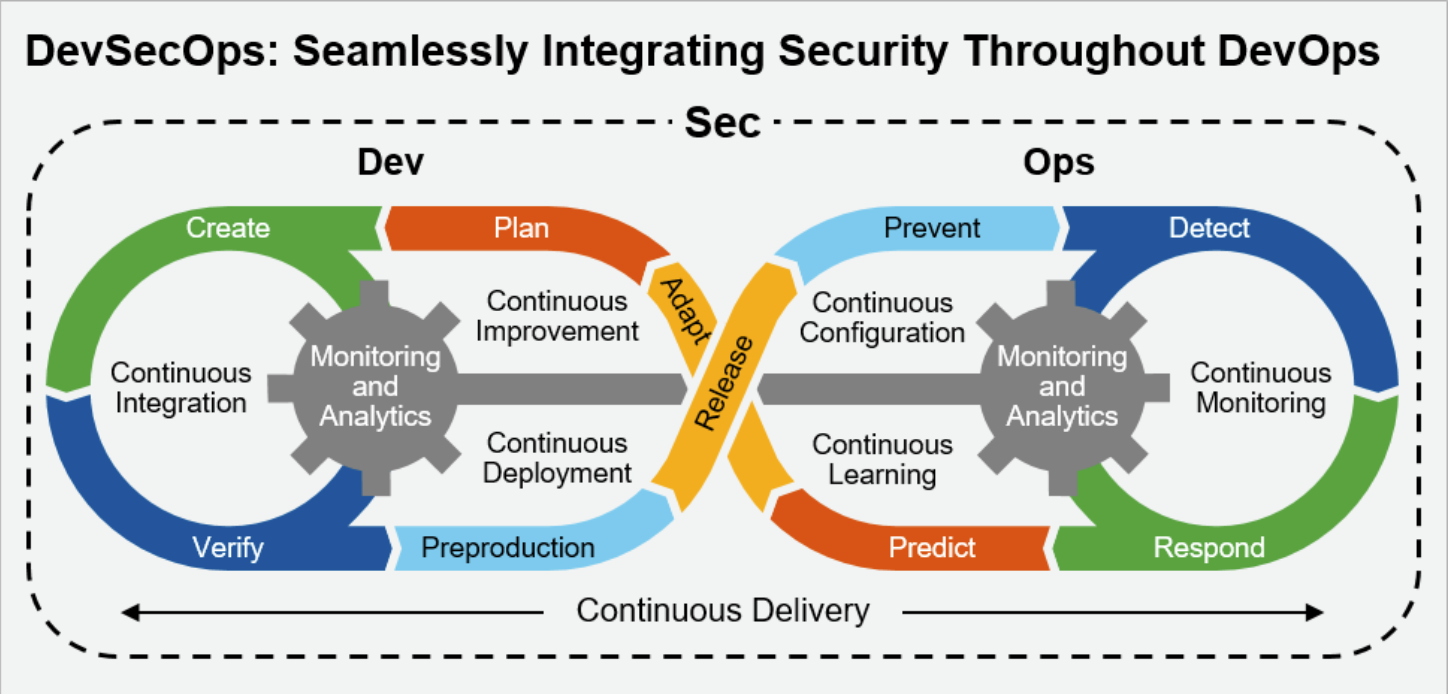
\includegraphics[width=\textwidth]{devsecops.png}

Como podemos observar en el gráfico anterior, el modelo de desarrollo basado en una filosofía DevSecOps, mueve las comprobaciones de seguridad desde la fase de mantenimiento, a la fase inicial, contemplando la seguridad como uno más de los requisitos que se plantean en la fase de planificación y conservando su importancia durante el resto de fases del proyecto.
En definitiva, la seguridad, pasa a ser una parte integral del ciclo de vida de desarrollo del software. 

Para conseguir este propósito, los practicantes de dicha filosofía implementan ``jobs'', o tareas automatizadas relacionadas con la seguridad en el mismo ``Pipeline'', tan característico de DevOps.

En los últimos años, el sector del software ha explotado con empresas como GitHub, GitLab o GoCD, que proporcionan a los equipos de desarrollo las herramientas básicas y los pilares fundamentales para que sus clientes adopten una filosofía DevOps y DevSecOps en la construcción de software.\cite{Google2019}

Un ejemplo de el uso de la filosofía DevSecOps es el concepto llamado ``Abuser storie'' \cite{Bor2006} en el que se aplica la seguridad en la fase de Planificación, a conceptos previos, como los ``User Stories''.

Un user story es una breve descripción escrita por el cliente de no más de tres líneas sobre la funcionalidad que debe proporcionar la aplicacion.  \cite{XPUserStory} mientras que un ``abuser story'' es una extension de los ``User Stories'' contemplado por un ingeniero de seguridad para poder tomar decisiones informadas en base al estado de la seguridad en el momento de su definición. \cite{Bor2006}

Esta forma de re plantearse la seguridad es exactamente el cambio de paradigma que lleva a la filosofía DevSecOps.


\chapter{Implementación del modelo DevSecOps}

El contenido de esta sección, define el problema al que nos enfrentamos, analizando los principales problemas con el pipeline actual en Scalefast.
Posteriormente, definiremos los objetivos a los que queremos llegar, detallando la razón por la cual se piensa que es el camino correcto en este momento para Scalefast.
Una vez definidos los objetivos, vamos a detallar el ciclo de desarrollo y puesta en producción de uno de nuestros objetivos detallados anteriormente para terminar redactando la conclusion a la que se ha llegado tras realizar este análisis del estado actual del pipeline y su subsecuente esfuerzo por evolucionarlo, de forma paralela a la dirección que esta llevando la industria.

\section{Análisis del estado actual del pipeline} %DEFINICIÓN DEL PROBLEMA

En Scalefast, se sigue un modelo de desarrollo similar al descrito anteriormente, en la metodología ágil.
Actualmente, la empresa tiene un pipeline de integración continua, en el que se pasan varios ``jobs'' o pruebas automáticas en cada commit vinculado a un \acrfull{mr} que se sube al repositorio de código.
Un pipeline es una pieza clave del ciclo de vida del software, responsable de asegurar la calidad de los desarrollos que integramos a producción y que por ende, definen la calidad de la empresa.
Dicho esto, es importante recordar que el desarrollo del pipeline debe seguir siempre el modelo de desarrollo de software que el mismo promueve, el desarrollo iterativo e incremental comprendido esto, es evidente que su desarrollo no tiene fin.
En vista de la progresión de Scalefast, debemos evolucionar el pipeline, haciendo que tienda mas hacia la integración y despliegues continuous, centrando ademas el desarrollo de software en la seguridad.
A medida que Scalefast ha crecido tanto en clientes, como en empleados y proyectos que abarcamos, se han identificado una serie de problemas con el pipeline que usamos actualmente.

\section{Definición de procesos}

Como se ha definido anteriormente, el objetivo principal de este trabajo es reciclar el pipeline que tenemos en funcionamiento actualmente en Scalefast por uno mas actual, que sea capaz de proporcionar a los equipos las herramientas y entornos que necesitan en el momento en el que las necesitan, de esta forma, podemos reducir el tiempo de desarrollo, aumentando ademas la calidad y seguridad del software que sacamos a producción.
De esta forma, Scalefast adquiere une ventaja competitiva injusta.

\subsection{Documentación y decision de procesos}

Como en cualquier proceso, para poder implementarlo en una empresa medianamente grande, hace falta la cooperación de varios responsables de equipo.
Este pipeline va a afectar tanto a los equipos de QA, como a los desarrolladores, como al equipo de Operaciones y Arquitectura.
En definitiva, toda la parte técnica de la empresa se va a ver afectada.
Es por esto que se debe tener en cuenta el punto de vista de todos los equipos mencionados anteriormente para que el resultado generado aporte beneficios a todos los equipos implicados.

\subsubsection{Análisis del pipeline desde el punto de vista de seguridad}

La creación del Pipeline require un proceso de análisis por parte de las distintas areas de la empresa.
En el equipo de seguridad, se ha optado por crear un pipeline conceptual, provisto de todas las herramientas necesarias para garantizar la seguridad de forma automática.
Partiendo de esa base, comparáramos el estado del pipeline actual y definimos una serie de perfiles, procesos y desarrollos necesarios para llevar a cabo el proyecto.
Posteriormente creamos el plan de desarrollo, exactamente igual que si se tratase de un proyecto de un cliente externo.



\section{DevSecOps en uso}

Recientemente, Mike Ensor y Drew Stevens publicaron un ``paper'' titulado ``Shifting left on security''.
En él, explican las diferentes fases de el ciclo de vida del software, y como añadir elementos de seguridad a lo largo del ``pipeline''. 
Desde la planificación del proyecto, hasta el despliegue del mismo.
Algunas de las técnicas que recomiendan en su ``paper'' tienen gran importancia, como el uso de registros privados, cuyas imágenes y recursos estén identificadas y sean verificadas a la hora de desplegarse, análisis estático y dinámico del código que se escribe de forma automatizada, despliegue del mismo binario, y que solamente pueda ser desplegado si es firmado de forma criptográfica por el responsable de despliegues.\cite{Ensor2021}

En esta sección, se describen mas en detalle dichas herramientas y se describe la implementación de alguna de ellas en el pipeline de Scalefast.

\clearpage

\printglossary[type=\acronymtype]

\printglossary

%----------
%	Bibliography
%----------	

\clearpage
\addcontentsline{toc}{chapter}{Bibliografía}

\printbibliography


%----------
%	Appendix
%----------	

% If your work includes Appendix, you can uncomment the following lines
%\chapter* {Appendix x}
%\pagenumbering{gobble} % Appendix pages are not numbered

\end{document}
